\def\x{{\bf x}}
\def\q{{\bf q}}
\def\p{{\bf p}}
\def\v{{\bf v}}

\lab{Fast Fourier Transform}{Fast Fourier Transform}
\objective{Explore how the Fourier transform applies to audio signals.}

\section*{Audio Signals}

In this lab we will be working with signals which represent sound.
First we should understand how sound is produced and transmitted.
As an example, consider a typical electronic speaker.

\begin{center}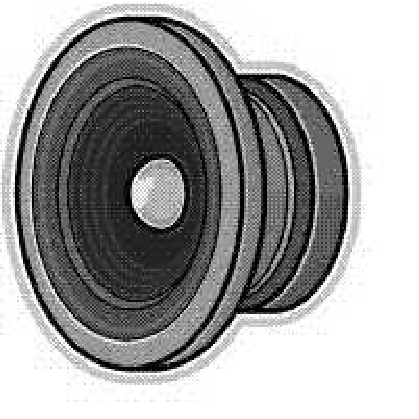
\includegraphics[width=45mm]{speaker}\end{center}
The essential component is a bowl-shaped membrane, called the \emph{cone} (or \emph{diaphragm}) of the speaker
A lightweight electromagnet is attached behind the cone.
When a current flows through the electromagnet in a certain direction, a magnetic field is created which repels the electromagnet (and the attached cone) from a heavier permanent magnet mounted behind it.
The cone thrusts forward, compressing the air in front of the speaker, resulting in a slight increase in air pressure which is propagated through the room in a wave.
When the direction of the current is reversed, the electromagnet is attracted to the permanent magnet.
The cone is pulled back, expanding the air in front of the speaker, resulting in a slight decrease in air pressure which, again, is propagated through the room in a wave.
These pressure waves reach your ears and are perceived as sound.
The basic mechanism of a speaker is entirely reversible; for instance, a pair of ordinary (non-amplifying) headphones can also, without any modification, be used as a stereo microphone (Try it!).


Play the audio clip \texttt{pulseramp.wav}.
You will hear a series of pulses, or clicks.
A click is a sudden (small) increase in pressure followed almost immediately by a return to normal pressure.
In a speaker, a click is produced by the cone suddenly thrusting forward a small amount and then gradually, silently, returning to its original position.
Notice that as the pulses occur closer and closer together, eventually your ears no longer perceive them as individual pulses.
Instead, they are perceived as a tone which increases in pitch as the pulses increase in frequency.

\begin{figure}[ht]\caption{A sequence of pulses of increasing frequency}\label{pulseramp}\centering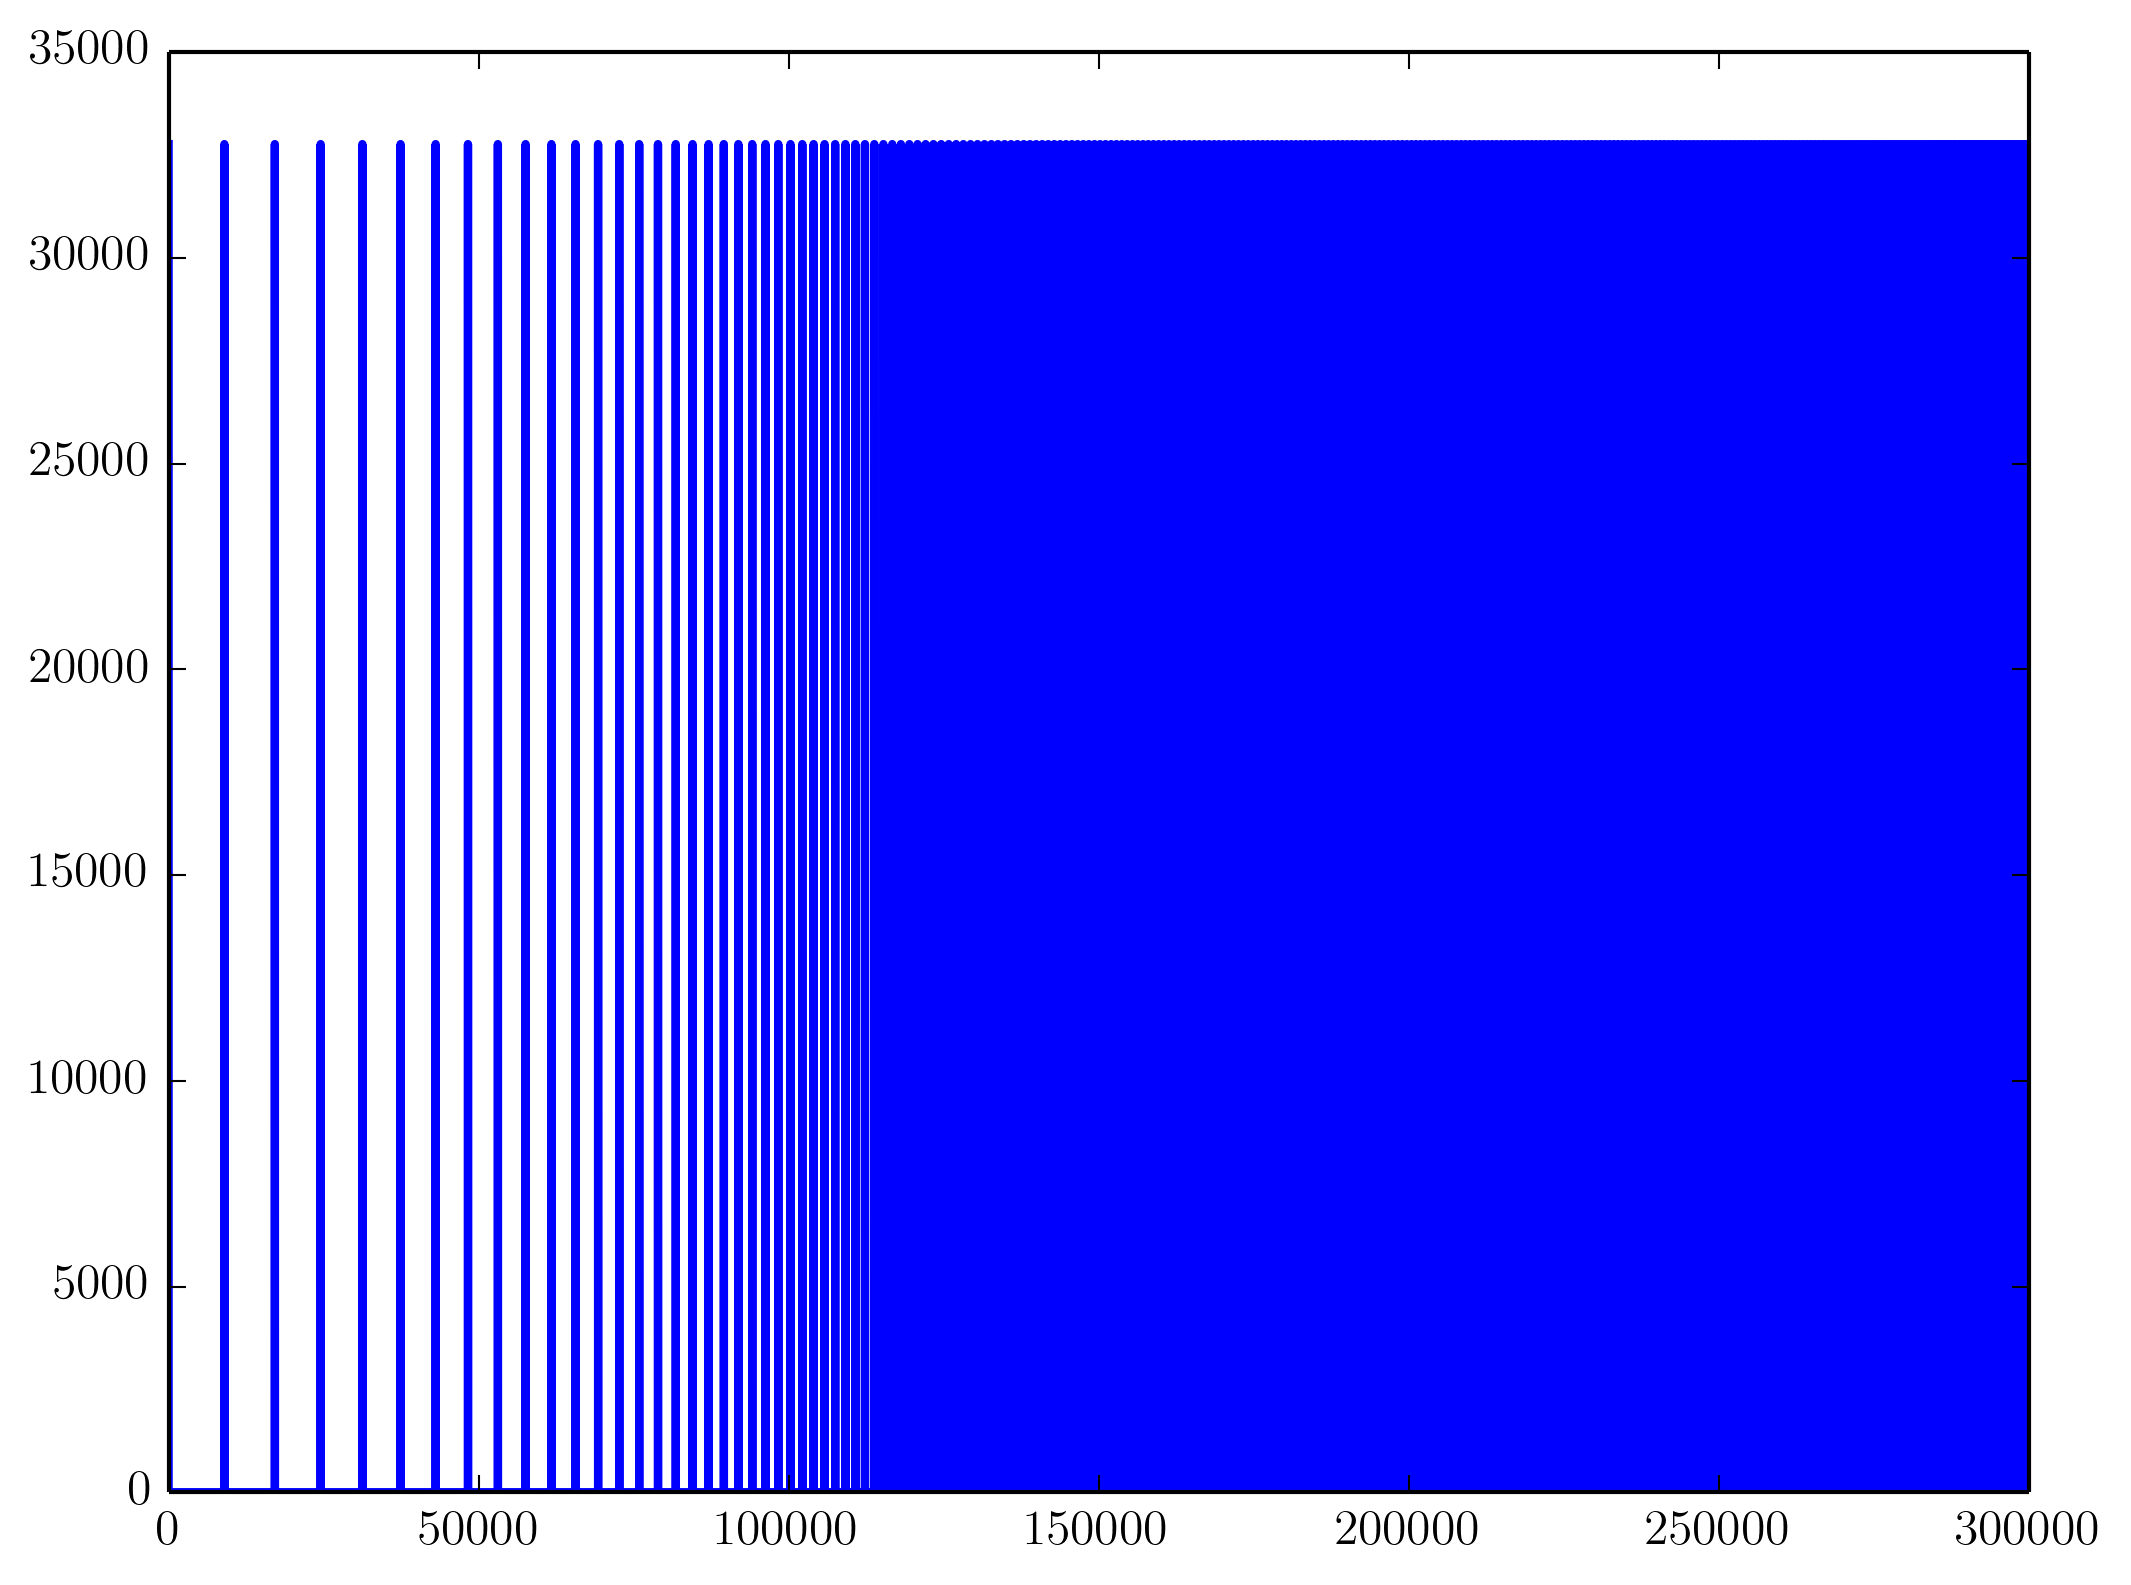
\includegraphics[width=\textwidth]{pulseramp}\end{figure}

In python we can read in a \texttt{.wav} by importing wavfile from \texttt{scipy.io} and using \texttt{wavfile.read()} as follows:
\begin{lstlisting}
import scipy as sp
from scipy.io import wavfile
from matplotlib import pyplot as plt

rate, mywave = wavfile.read('pulseramp.wav')
\end{lstlisting}

Here \texttt{mywave} is the signal and \texttt{rate} is the sampling rate of the audio measured in Hz (samples per second).
In this case, \texttt{mywave} is a vector of length $300000$.
It has only one column because this is a mono (single-channel) \texttt{.wav} file.
If we had used a stereo \texttt{.wav} file, then \texttt{mywave} would have been a matrix with two columns, one for the left channel and one for the right.

The entries of \texttt{mywave} are integers between $-32767$ and $+32767$ representing the relative air pressure at a particular instant, sampled at regular intervals (these bounds are the range of 16-bit integers).
In our case, the \texttt{.wav} file is sampled at 44.1KHz (the standard sample-rate for high-quality audio), so there are 44100 samples per second. 
$+32767$ represents the maximum possible increase in air pressure which the speaker can produce (at its current volume level), while $-32767$ represents the maximum possible decrease in air pressure.
In the case of our particular \texttt{.wav} file, you can check that most of the entries of \texttt{mywave} are $0$, indicating neutral pressure. 
Only occasionally you will find an entry which is $+32767$, which is where a pulse occurs.
We can see this most easily if we plot the waveform of our sound (see Figure \ref{pulseramp}):
\begin{lstlisting}
plt.plot(mywave)
plt.show()
\end{lstlisting}

We should keep in mind that the deviations in air pressure that we hear as sound are extremely small relative to atmospheric pressure.
In normal conversation the deviation in air pressure reaching your ears might be around $.01$ pascals, about one ten-millionth of atmospheric pressure.


\section*{The Spectrum of a Signal}

In many ways the most basic kind of sound is one whose waveform is a sinusoid (that is, a scaled, shifted version of the sine function). 
To the ear, the tone of a sinusoid is more mellow than any other sound of the same pitch. 
Mathematically sinusoids are important because Fourier series provide a way of expressing any periodic, piecewise continuous function as a sum of sine and cosine waves of various frequencies and amplitudes, or, more conveniently, using complex exponential functions.

Here's one way of producing a 1760Hz sine wave (which in musical terms is A6, the A between two and three octaves above middle C):

\begin{lstlisting}
samplerate = 44100	# 44100 samples per second
freq = 1760			# Produce a 1760 Hz sine wave ...
length = 2			# ... which lasts for 2 seconds.
stepsize = freq * 2 * sp.pi/samplerate
sig = sp.sin(sp.arange(0, stepsize*length*samplerate, stepsize))
scaled = sp.int16(sig/sp.absolute(sig).max() * 32767) # Scale the wave
wavfile.write('sinusoid.wav', samplerate, scaled)
\end{lstlisting}

Notice before writing the file we had to scale it to be a 16-bit integer between -32767 and +32767 because \texttt{wavfile.write()} expects the data to be in this form.

\begin{problem} % Problem 1
Write a function that plots the signal of any given \texttt{.wav} file. Generate a 60Hz sine wave 1 second in length, save it as a \texttt{.wav} file, and use your function to plot the signal. Play the resulting file (\textbf{Warning}: turn down your volume!).
\end{problem}


For a discrete signal, we are given a finite number of evenly spaced data points along the $x$-axis; we can think of such a signal as a function $f$ whose domain consists of the integers $\{0,1,\dots,N-1\}$, where $N$ is the number of data points. 
We often extend $f$ to be a periodic function with period $N$, defined on all integers, by requiring $f(a+bN)=f(a)$ for all integers $a$ and $b$.
How might we find something analagous to a Fourier series for such a function?
It turns out that the functions $e^{\frac{2\pi ikx}N}$, which are periodic with period $N$, form an orthonormal set with respect to the inner product
\[
\langle f,g\rangle = \frac1N\sum_{k=0}^{N-1}\overline{f(k)}g(k).
\]
In particular, these functions are linearly independent and hence form a basis for the $N$-dimensional (complex) vector space of complex-valued functions with domain $\{0,\dots,N-1\}$.
The vector of coordinates of a function $f$ with respect to this basis constitutes what is called the \emph{discrete Fourier transform} (or \emph{DFT}) of the function $f$.
In other words, any function $f$ whose domain consists of the integers $\{0,1,\dots,N-1\}$ may be written in the form
\[
f(x)=\sum_{k=0}^{N-1}c_ke^{\frac{2\pi ikx}N}.
\]
The vector of coefficients $(c_0,c_1,\dots,c_{N-1})$ is called the DFT of $f$. These coefficients may be computed by taking the inner product of each basis function with $f$:
\begin{align}
	c_k=\langle e^{\frac{2\pi ikx}N}, f(x)\rangle=\frac1N\sum_{n=0}^{N-1}e^{\frac{-2\pi ikn}N}f(n) . \label{transform_coefficients}
\end{align}


Scipy contains a module called \texttt{fft} which can compute the DFT of a signal.
For example, take the sine wave signal \texttt{sig} created above and run
\begin{lstlisting}
from scipy import fft

fsig = fft(sig)
\end{lstlisting}
Here \texttt{fsig} is an array of complex numbers representing the DFT of this signal. We plot the absolute values of the entries of \texttt{fsig} in Figure \ref{sinespec}.

Notice that there are two spikes, one on the left and one on the right.
Why are there two spikes when there is only one tone?
The answer is that for a real-valued signal, the right half of the DFT is always a mirror-image duplicate of the left half -- or, more precisely, each entry in the right half of the DFT is the complex conjugate of the corresponding entry in the left half.
Thus the right half of the DFT gives us no new information.
(To be completely accurate in describing this mirror-image symmetry, we must ignore the very first entry of the DFT.)


\begin{problem} % Problem 2
Implement a function to compute the DFT of a vector by using \eqref{transform_coefficients}.
Remember to use complex arrays in your computations (set \texttt{dtype=sp.complex128} when creating a scipy array, etc.).
For each coefficient $c_k$, can you implement the sum in a single line of code?

Test your function on several random vectors (representing the vector $[f(0),f(1),\dots,f(N-1)]$ and make sure the results match those of scipy's \texttt{fft}. 
Note that the scaling scipy uses does not divide by $N$, so be sure to account for that in your comparison.
\end{problem}


\begin{figure}[ht]\caption{DFT of a sine wave}\label{sinespec}\centering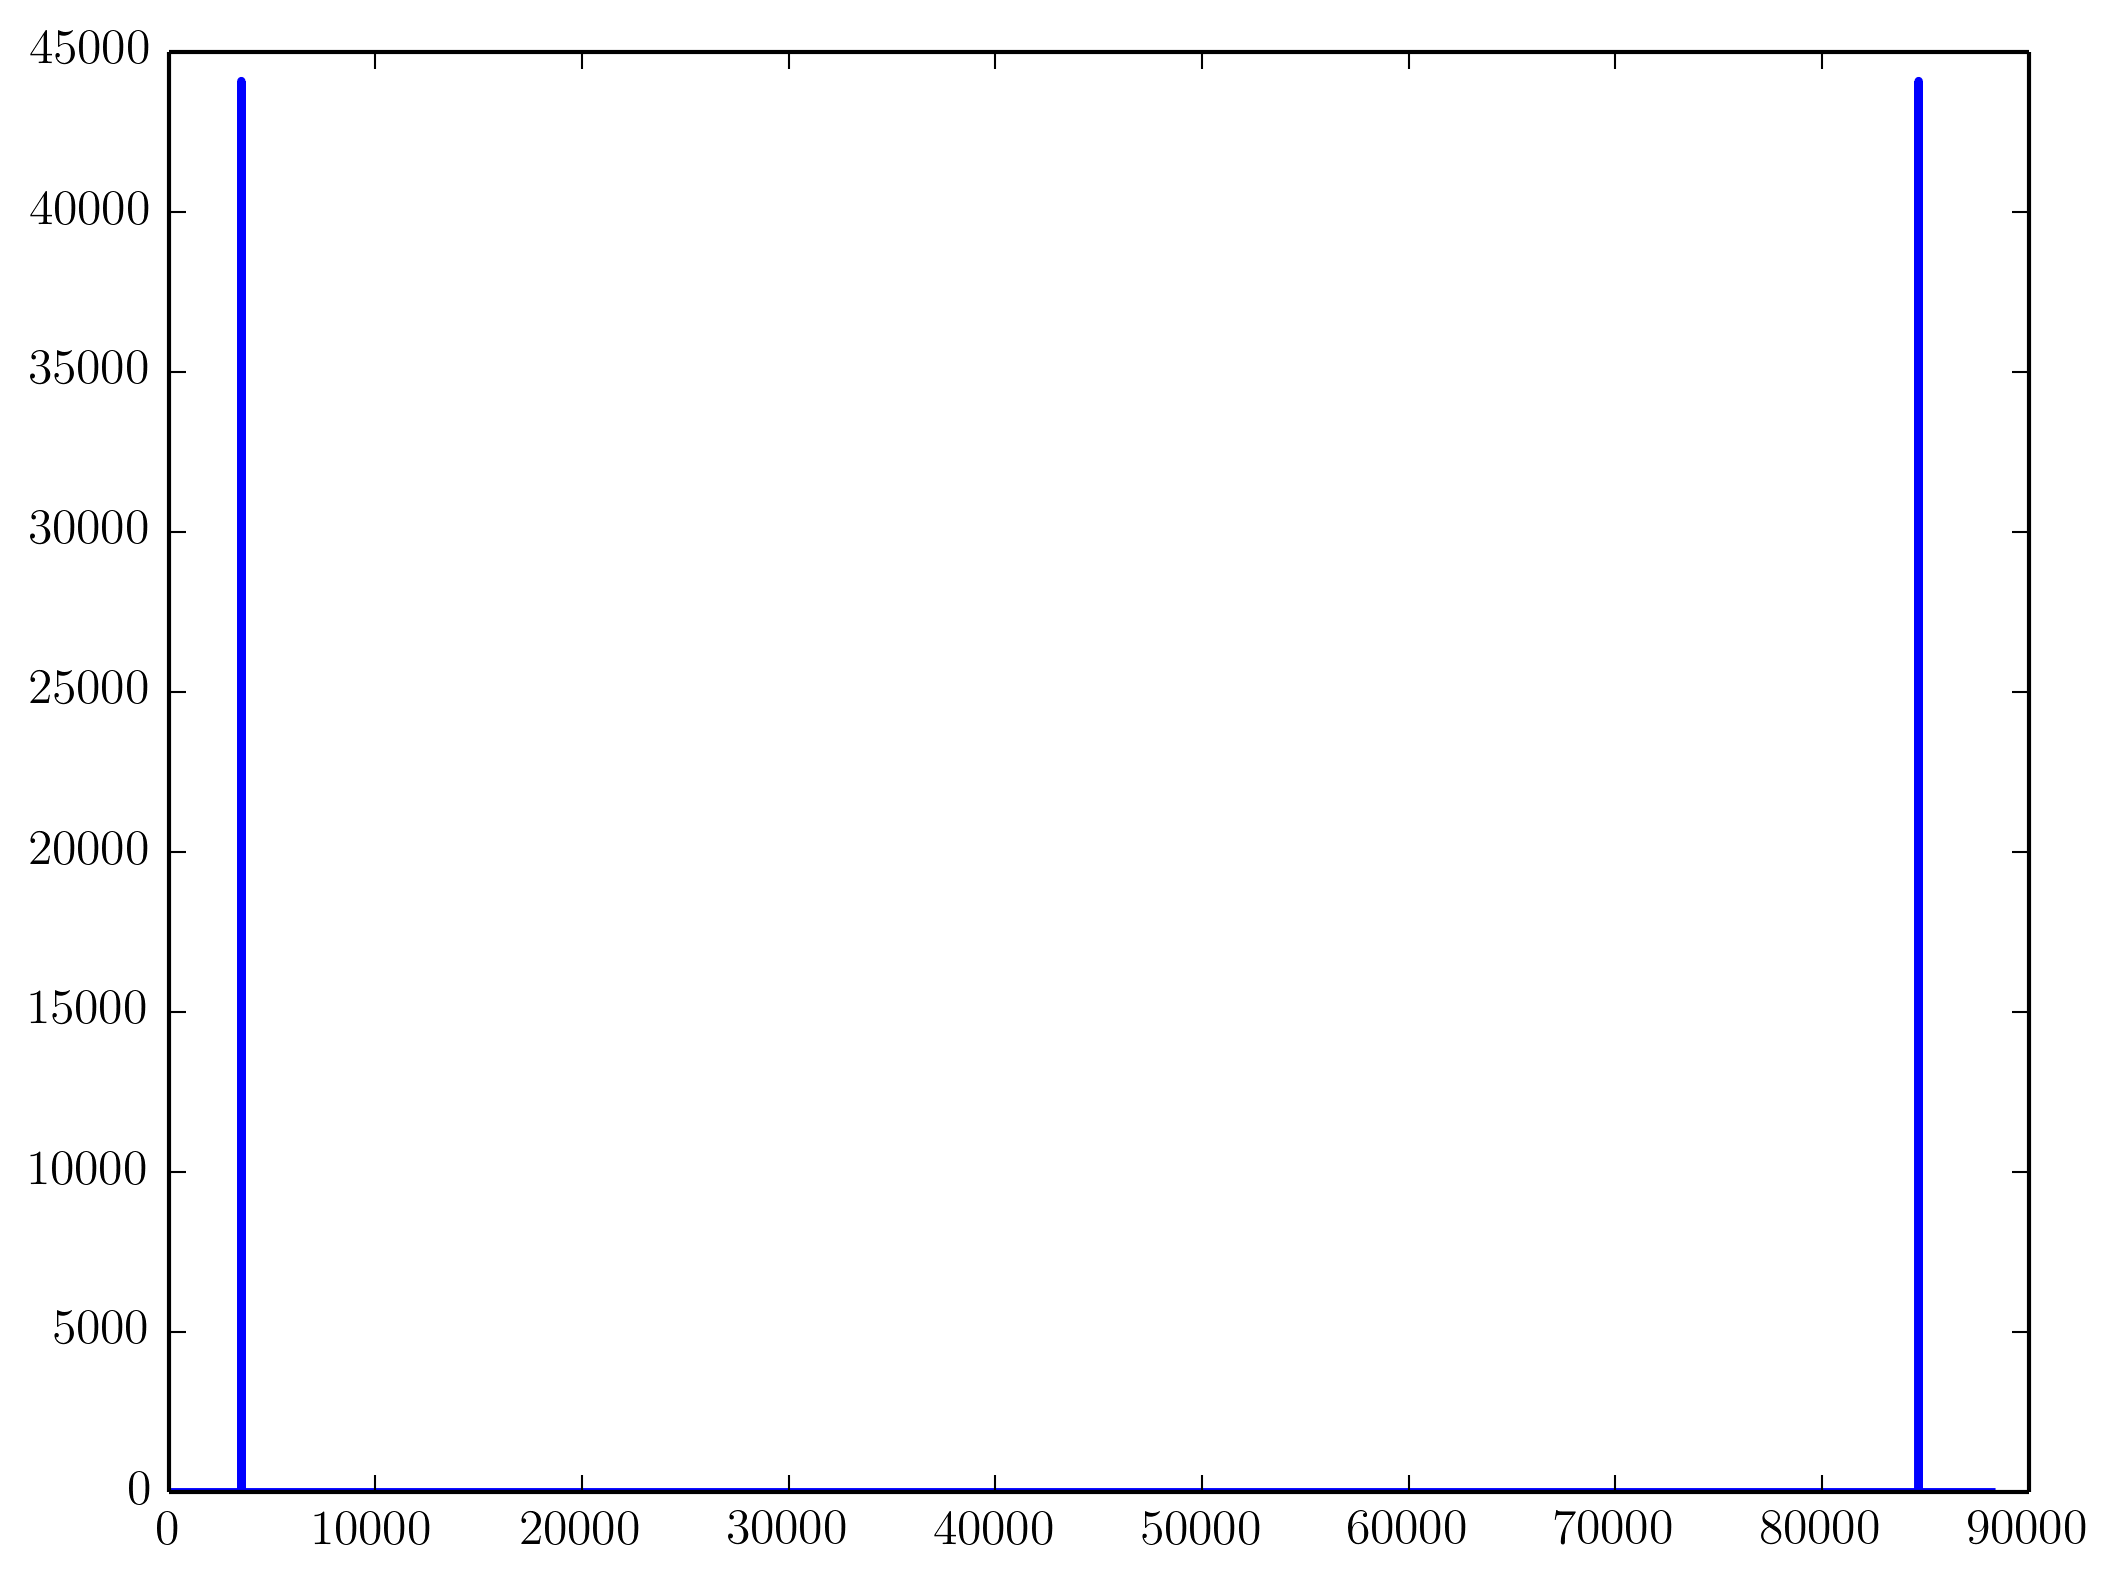
\includegraphics[width=\textwidth]{sinespec}\end{figure}

The naive way of computing the DFT has $O(N^2)$ runtime.
There is a very important algorithm which computes the DFT with a $O(N \log N)$ runtime, called the \emph{fast Fourier transform}.
The fast Fourier transform (FFT) accomplishes this speedup by recursively breaking up the original array into smaller pieces, finding the Fourier transform of those smaller pieces, and carefully recombining to get the Fourier transform of the original array.
While scipy uses the FFT algorithm, its implementation at the time of this writing is still somewhat slow.

However, there is a $C$ library that computes the FFT called FFTW (Fastest Fourier Transform in the West).
A python package called ``pyFFTW'' wraps FFTW and is available for download. %%% WHERE!?!?!?
pyFFTW  has an interface to FFTW called scipy\_fftpack that acts exactly like scipy's fft, but it is substantially faster than scipy's implementation when processing larger arrays.

Now let's look at a more complicated signal. Play the file \texttt{tada.wav}.
If you read \texttt{tada.wav} into python you will find it has two columns.
That is because it is a stereo recording; the two columns correspond to two audio signals (left and right).
By default, pyFFTW takes the Fourier transform along the last axis. We override this by setting axis=0.

The following code computes the discrete Fourier transform of \texttt{tada.wav} and graphs its absolute values (see Figure \ref{tadaspec}).

\begin{figure}[ht]\caption{Absolute value of the DFT of \texttt{tada.wav}}\label{tadaspec}\centering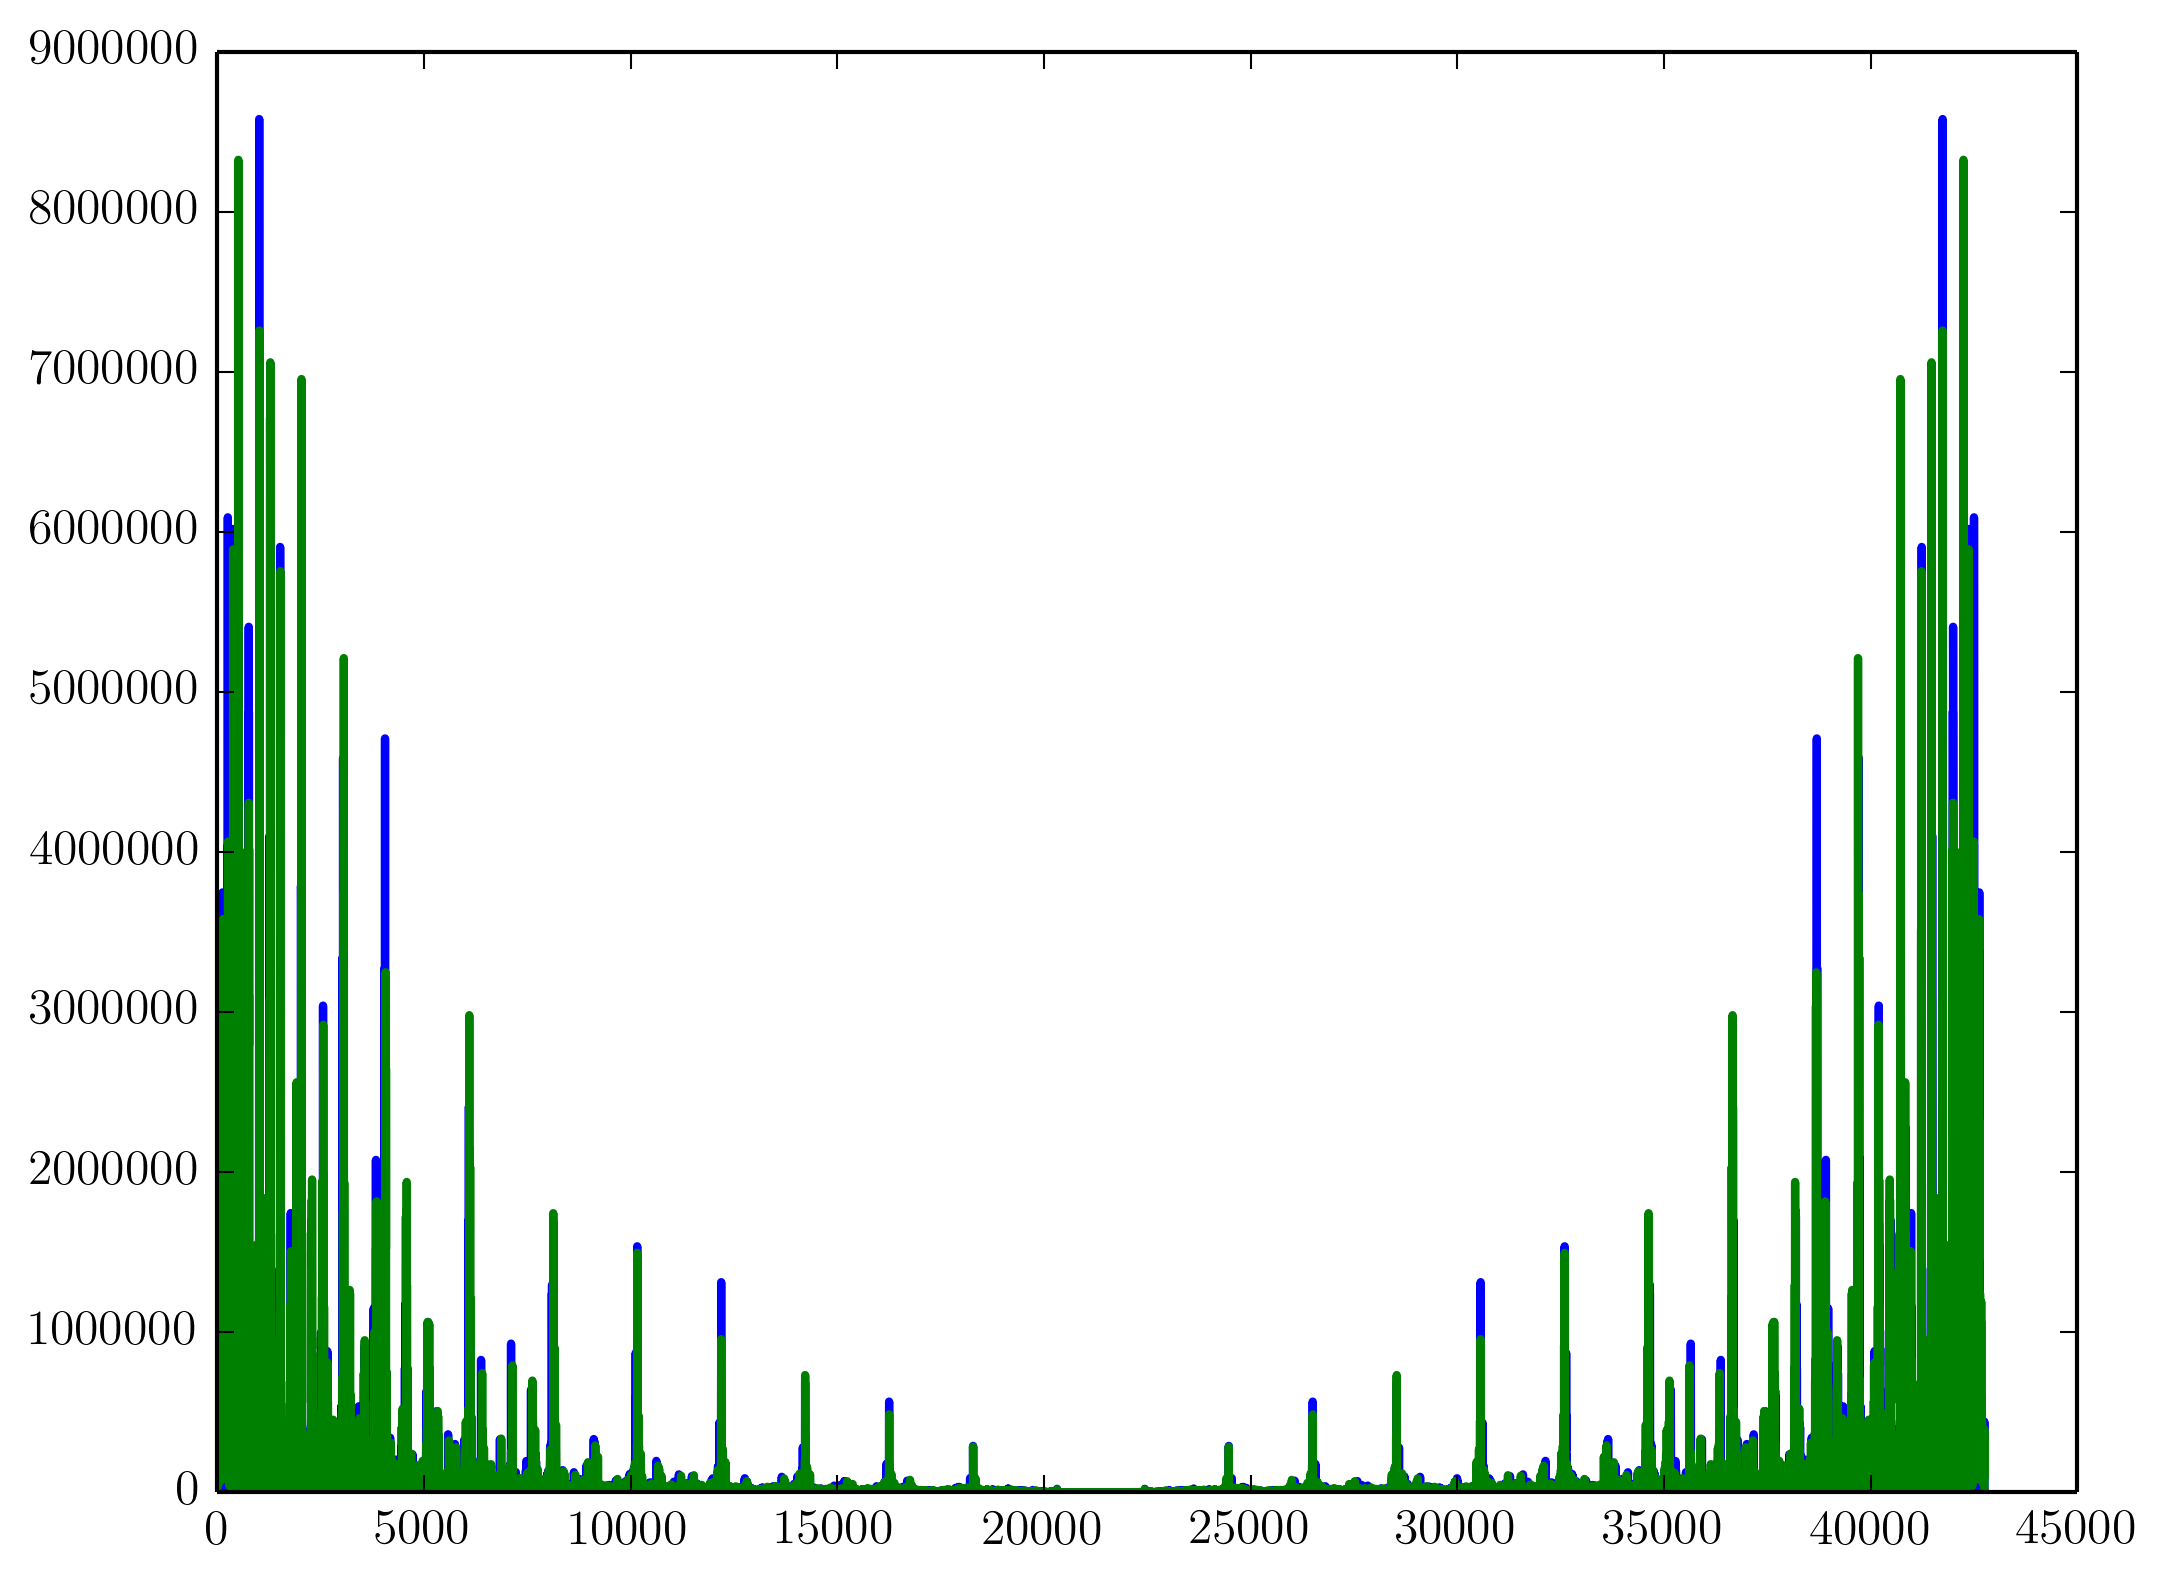
\includegraphics[width=\textwidth]{tadaspec}\end{figure}

\begin{lstlisting}
from pyfftw.interfaces import scipy_fftpack as fftw
rate, sig = wavfile.read('tada.wav')
sig = sp.float32(sig)
fsig = fftw.fft(sig,axis=0)
plt.plot(sp.absolute(fsig))
plt.show()
\end{lstlisting}


Again, the right half of the plot is a mirror-image duplicate of the left half.
We might as well exclude it by only plotting the left half.
The absolute value of the left half of  the DFT is called the \emph{spectrum} of the signal (see Figure \ref{tadaspec2}):
\begin{lstlisting}
f = sp.absolute(fsig)
plt.plot(f[0:f.shape[0]/2,:])
plt.show()
\end{lstlisting}
\begin{figure}[ht]\caption{Spectrum of \texttt{tada.wav} (Absolute value of left half of DFT)}\label{tadaspec2}\centering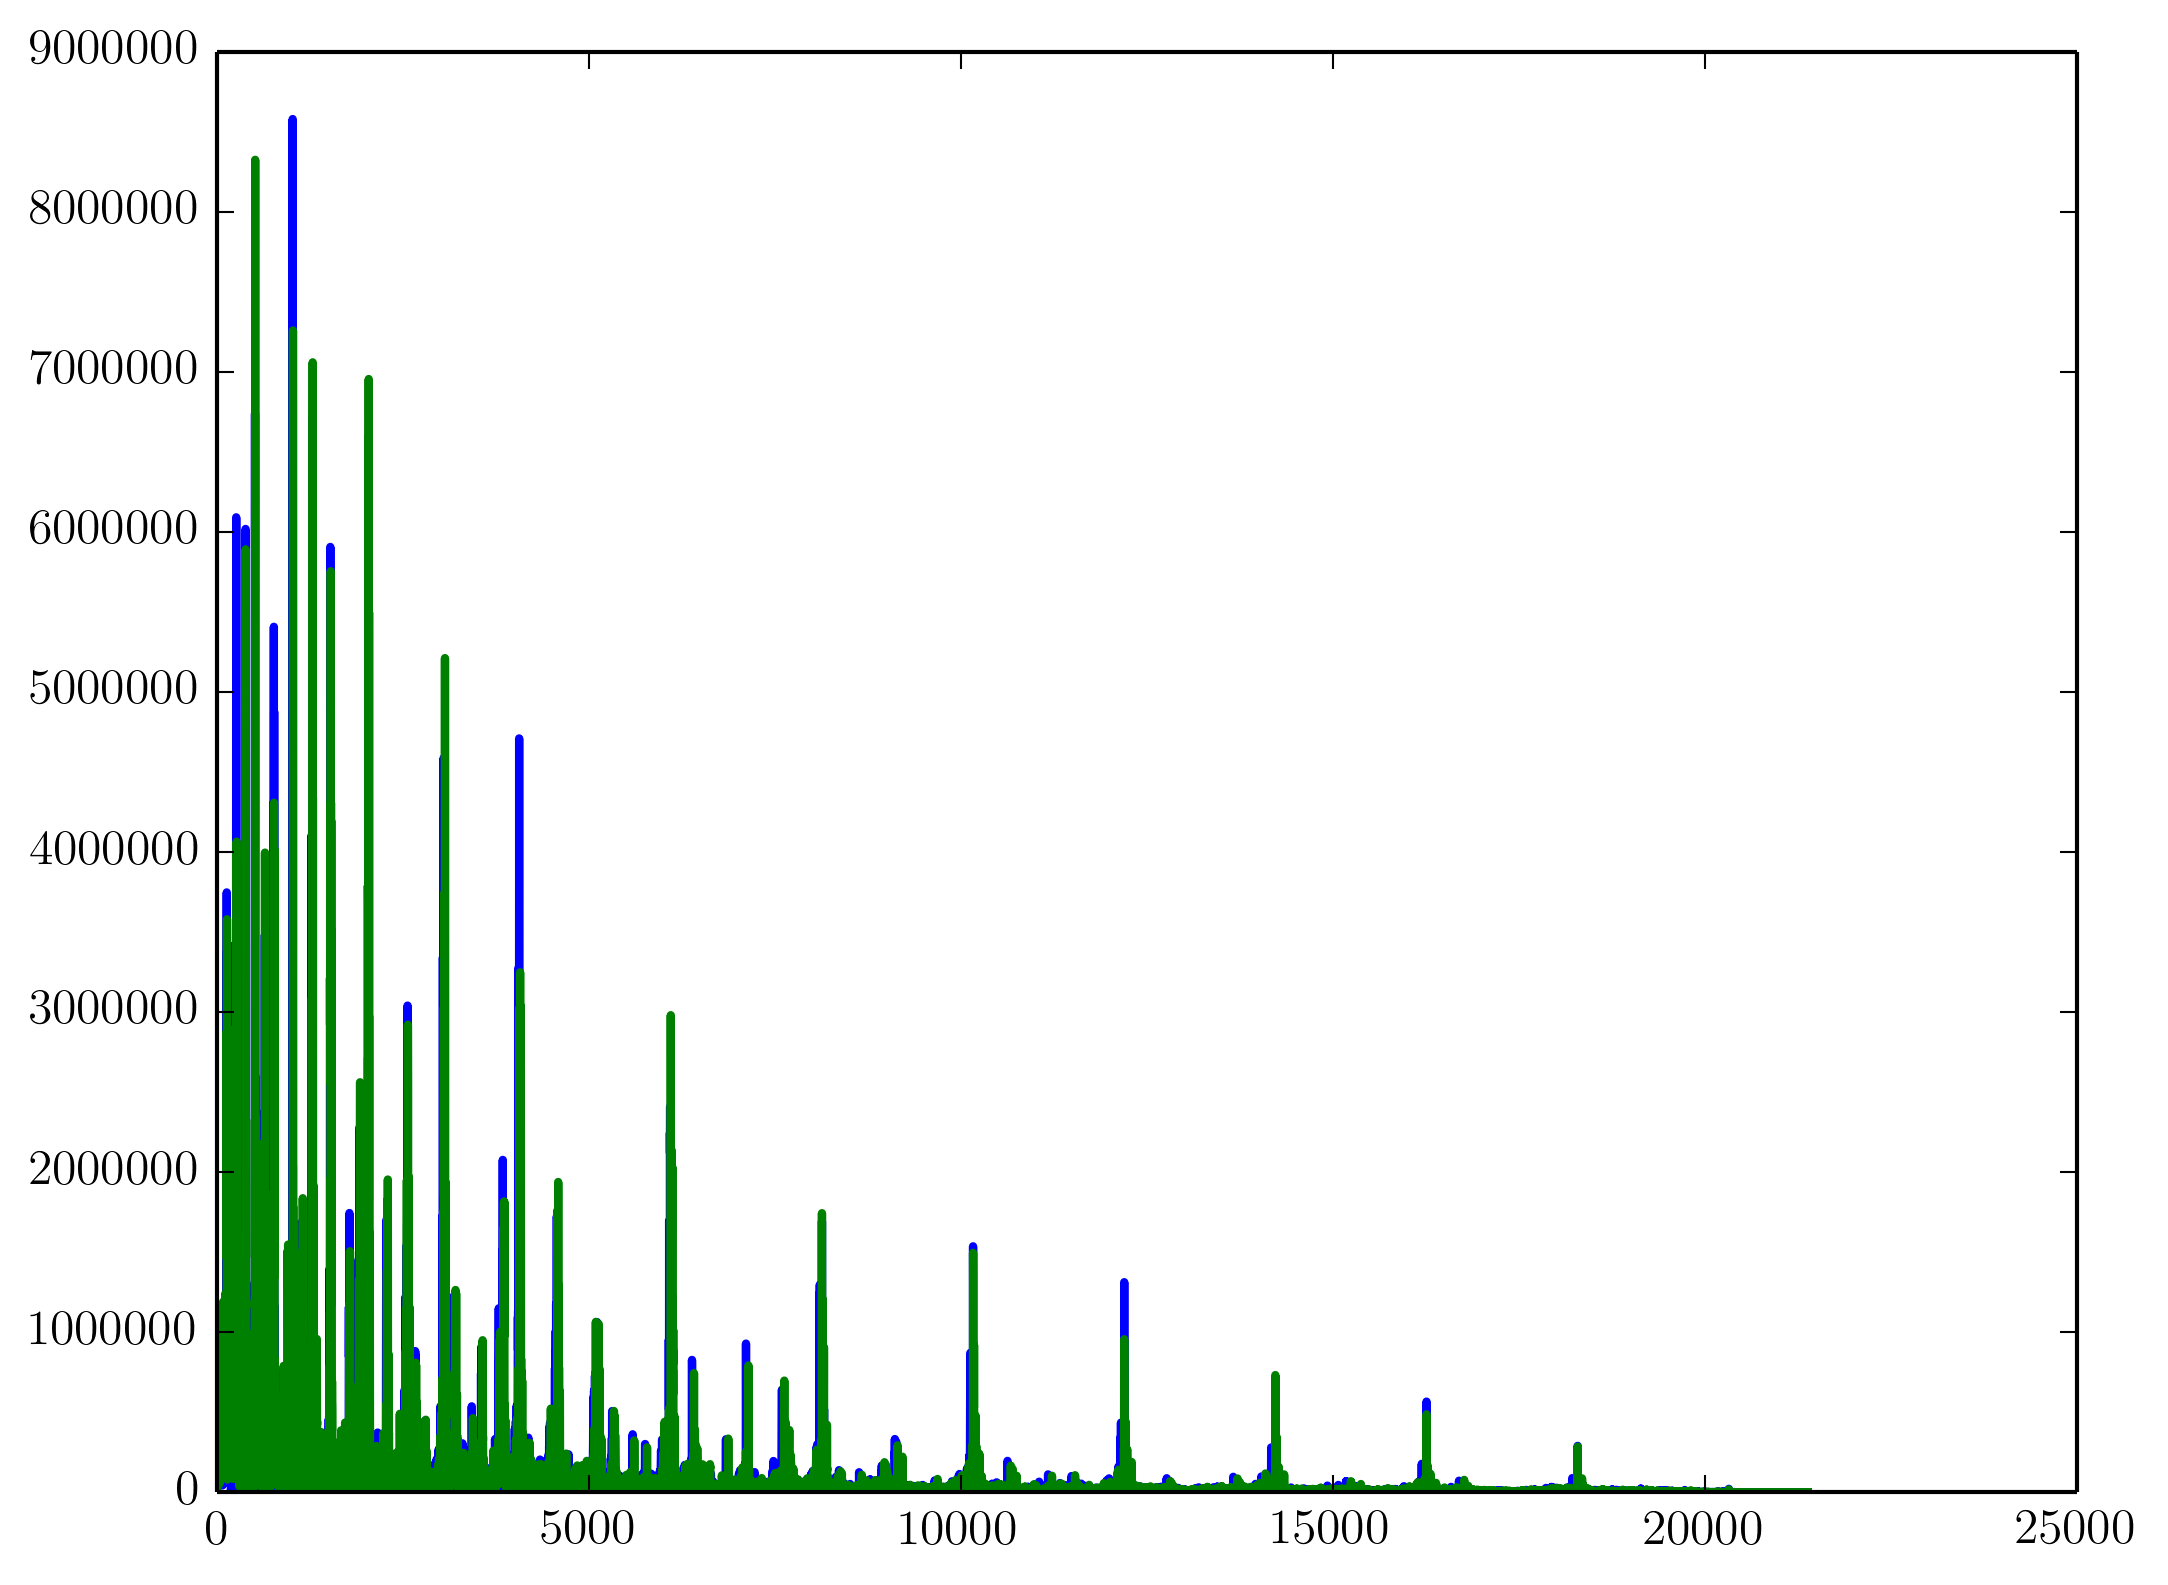
\includegraphics[width=\textwidth]{tadaspec2}\end{figure}
Notice that the number of spikes in the plot is much greater than the number of musical notes in the sound: whenever a note is played on a musical instrument, more than one frequency is produced.
The lowest frequency is called the \emph{fundamental}, and the others, which usually occur as integer multiples of the fundamental frequency, are called \emph{overtones}.
In instruments with a mellow tone (such as a flute or vibraphone) the overtones are relatively soft, while in instruments with a brighter tone (such as a trumpet) the overtones are quite prominent.
In the DFT of \texttt{tada.wav}, you will notice spikes at about 2030, 4060, 6090, 8120, 10160, 12190, 14220, 16250, 18280, and 20320 units.
These are approximately integer multiples of 2030 and represent overtones of a single musical note whose fundamental frequency is about 2030 units.

So what are these units and how can we express them in Hz? 
A frequency of 2030 units in the DFT means that the tone undergoes 2030 cycles through the extent of the entire recording. 
% We use check the shape of \texttt{sig} to find the total number of samples in the recording:
% \begin{verbatim}
% sig.shape
% Out[27]: (42752, 2)
% \end{verbatim}
% So the entire recording is 42752 samples long (in each channel -- this is a stereo recording.) 
Since \texttt{sig.shape}$\, = (42752, 2)$, we see that the entire recording is 42752 samples long in 2 channels (this is a stereo recording).
The sample rate is 22050 samples per second.
(You could find this out, for instance, by looking at the rate value assigned by \texttt{wavfile.read}). 
Thus, 2030 cycles through the entire recording is equivalent to
$$\frac{2030\text{ cycles}}{42752\text{ samples}} \times \frac{22050\text{ samples}}{\text{sec}} \approx 1043 \text{ Hz}.$$
This tone is at 1043 Hz, which in musical terms is a very slightly flat (concert) C6, the C two octaves above middle C.
There are also other, lower musical notes in the recording which each have their own sequence of overtones.

\begin{problem} % Problem 3
Listen to \texttt{pianoclip.wav}.
Use the DFT to identify the audible frequency of greatest amplitude, ignoring the 0 frequency found in the first entry (hint: use \texttt{sp.argmax()} to find the exact frequency).
What musical note does the fundamental frequency correspond to?
(Use the table on http://en.wikipedia.org/wiki/Piano\_key\_frequencies)
\end{problem}

You will notice that in this case the largest spike actually occurs in the very first entry of the DFT.
This corresponds to a frequency of 0Hz.
%A cosine wave of 0Hz is nothing other than a constant function.
%The presence of this 0Hz frequency, if taken literally, would mean that there was a (slight) sustained increase above the normal atmospheric pressure throughout the recording.
%However, a speaker or musical instrument, because of its bounded ranges of motion, is incapable of producing a sustained increase (or decrease) in pressure; and a microphone, for the same reason, is incapable of detecting such a sustained change in pressure.
%An ordinary speaker cannot produce frequencies below about 15 to 20Hz, and even if it could, we would not be able to hear them.
The 0Hz frequency which appears here is simply an artifact of an imperfect recording device.
It indicates that some direct current ``leaked" through the device.



\section*{Down-sampling a signal}

Listen to \texttt{saw.wav}.
You will hear a high-pitched buzzing sound \footnote{The technical term for it is a sawtooth wave; for the curious, see http://en.wikipedia.org/wiki/Sawtooth\_wave}.
The sound is recorded at a sample rate of 44.1KHz.
Now let's say we wanted to convert it to a 22.05KHz sample rate.
Since we're cutting the sample rate in half, we might think that we could accomplish this simply by discarding every other sample, i.e., keep the even-index samples and discard the odd-index samples.
Let's try that and see how it works:
\begin{lstlisting}
rate, in_sig = wavfile.read('saw.wav')
out_sig = in_sig[sp.arange(0, rate, 2)]
wavfile.write('down_saw.wav', rate / 2, out_sig)
\end{lstlisting}
The resulting signal sounds much like the original except that there are some extra tones which weren't there to begin with; these extra tones, in this case, are not in a nice harmonic relationship with the original tone and clash rather badly.
One of the extra tones is at a frequency of about 99Hz, which is rather low compared to the 1568Hz of the fundamental frequency in the original tone.
Where are these mysterious ``extra" tones coming from?

To explain this, we need to understand some important facts about sampling.
First of all, a basic fact is that the highest possible frequency that a sampled signal can represent is half the sampling rate.
Such a frequency is represented by alternating between +32767 and -32767 at each sample.
This frequency is known as the \emph{Nyquist frequency}.
If, for instance, the sampling rate is 44.1KHz, then the Nyquist frequency will be 22.05KHz.
This is slightly beyond the upper limit of human hearing; thus, for audio, generally no improvement in quality results from using a higher sampling rate than 44.1KHz, since at 44.1KHz the entire audible spectrum can already be represented.

Now let's consider what would happen if we tried to represent a frequency beyond the Nyquist frequency.
We create a sinusoid of frequency $f$ Hz by setting
$$s_k = \cos\left(\frac{2\pi kf}r\right)$$
where $s_k$ is the value of the $k$th sample and $r$ is the sample rate in Hz.
Suppose we take the frequency to be $f=\frac{r}2+a$, where $a$ is some positive number, so that $f$ is beyond the Nyquist frequency.
Then we have
\begin{align*}
s_k &= \cos\left(\frac{2\pi kf}r\right) \\
&= \cos\left(\frac{2\pi k(\frac{r}2+a)}r\right)\\
&= \cos\left(\pi k+\frac{2\pi ka}r\right)\\
&= \cos\left(-\left(\pi k+\frac{2\pi ka}r\right)\right)\\
&= \cos\left(-\left(\pi k+\frac{2\pi ka}r\right)+2\pi k \right)\\
&= \cos\left(\pi k-\frac{2\pi ka}r\right)\\
&= \cos\left(\frac{2\pi k(\frac{r}2-a)}r\right).
\end{align*}
But this is a sinusoid of frequency $\frac{r}2-a$, which is a frequency below the Nyquist frequency.
Thus a sinusoid above the Nyquist frequency, when sampled, is indistinguishable from a corresponding sinusoid below the Nyquist frequency.
An electronic speaker, given the sampled signal, will actually produce the sinusoid which lies below the Nyquist frequency, not the one above.
Thus, \emph{a frequency above the Nyquist frequency will, when sampled, have its frequency reflected across the Nyquist frequency.}
This phenomenon is known as \emph{aliasing}.

What does this have to do with our problem?
Our tone is at 1568Hz, which is well below the Nyquist frequency of 22050Hz.
However, there are prominent overtones extending all the way up to 21951Hz (see Figure \ref{sawspec})
Since we are downsampling to 22050Hz, the new Nyquist frequency will be 11025Hz.
The overtones in our signal which lie between 11025Hz and 22050Hz will then be reflected across the new Nyquist frequency in our downsampled sound.
For example, the overtone at 21951Hz will be reflected to $11025-(21951-11025)=99$ Hz, the lowest ``extra" tone that we observed.
See Figure \ref{sawspecdown}.

\begin{figure}[ht]\caption{Spectrum of \texttt{saw.wav}}\label{sawspec}\centering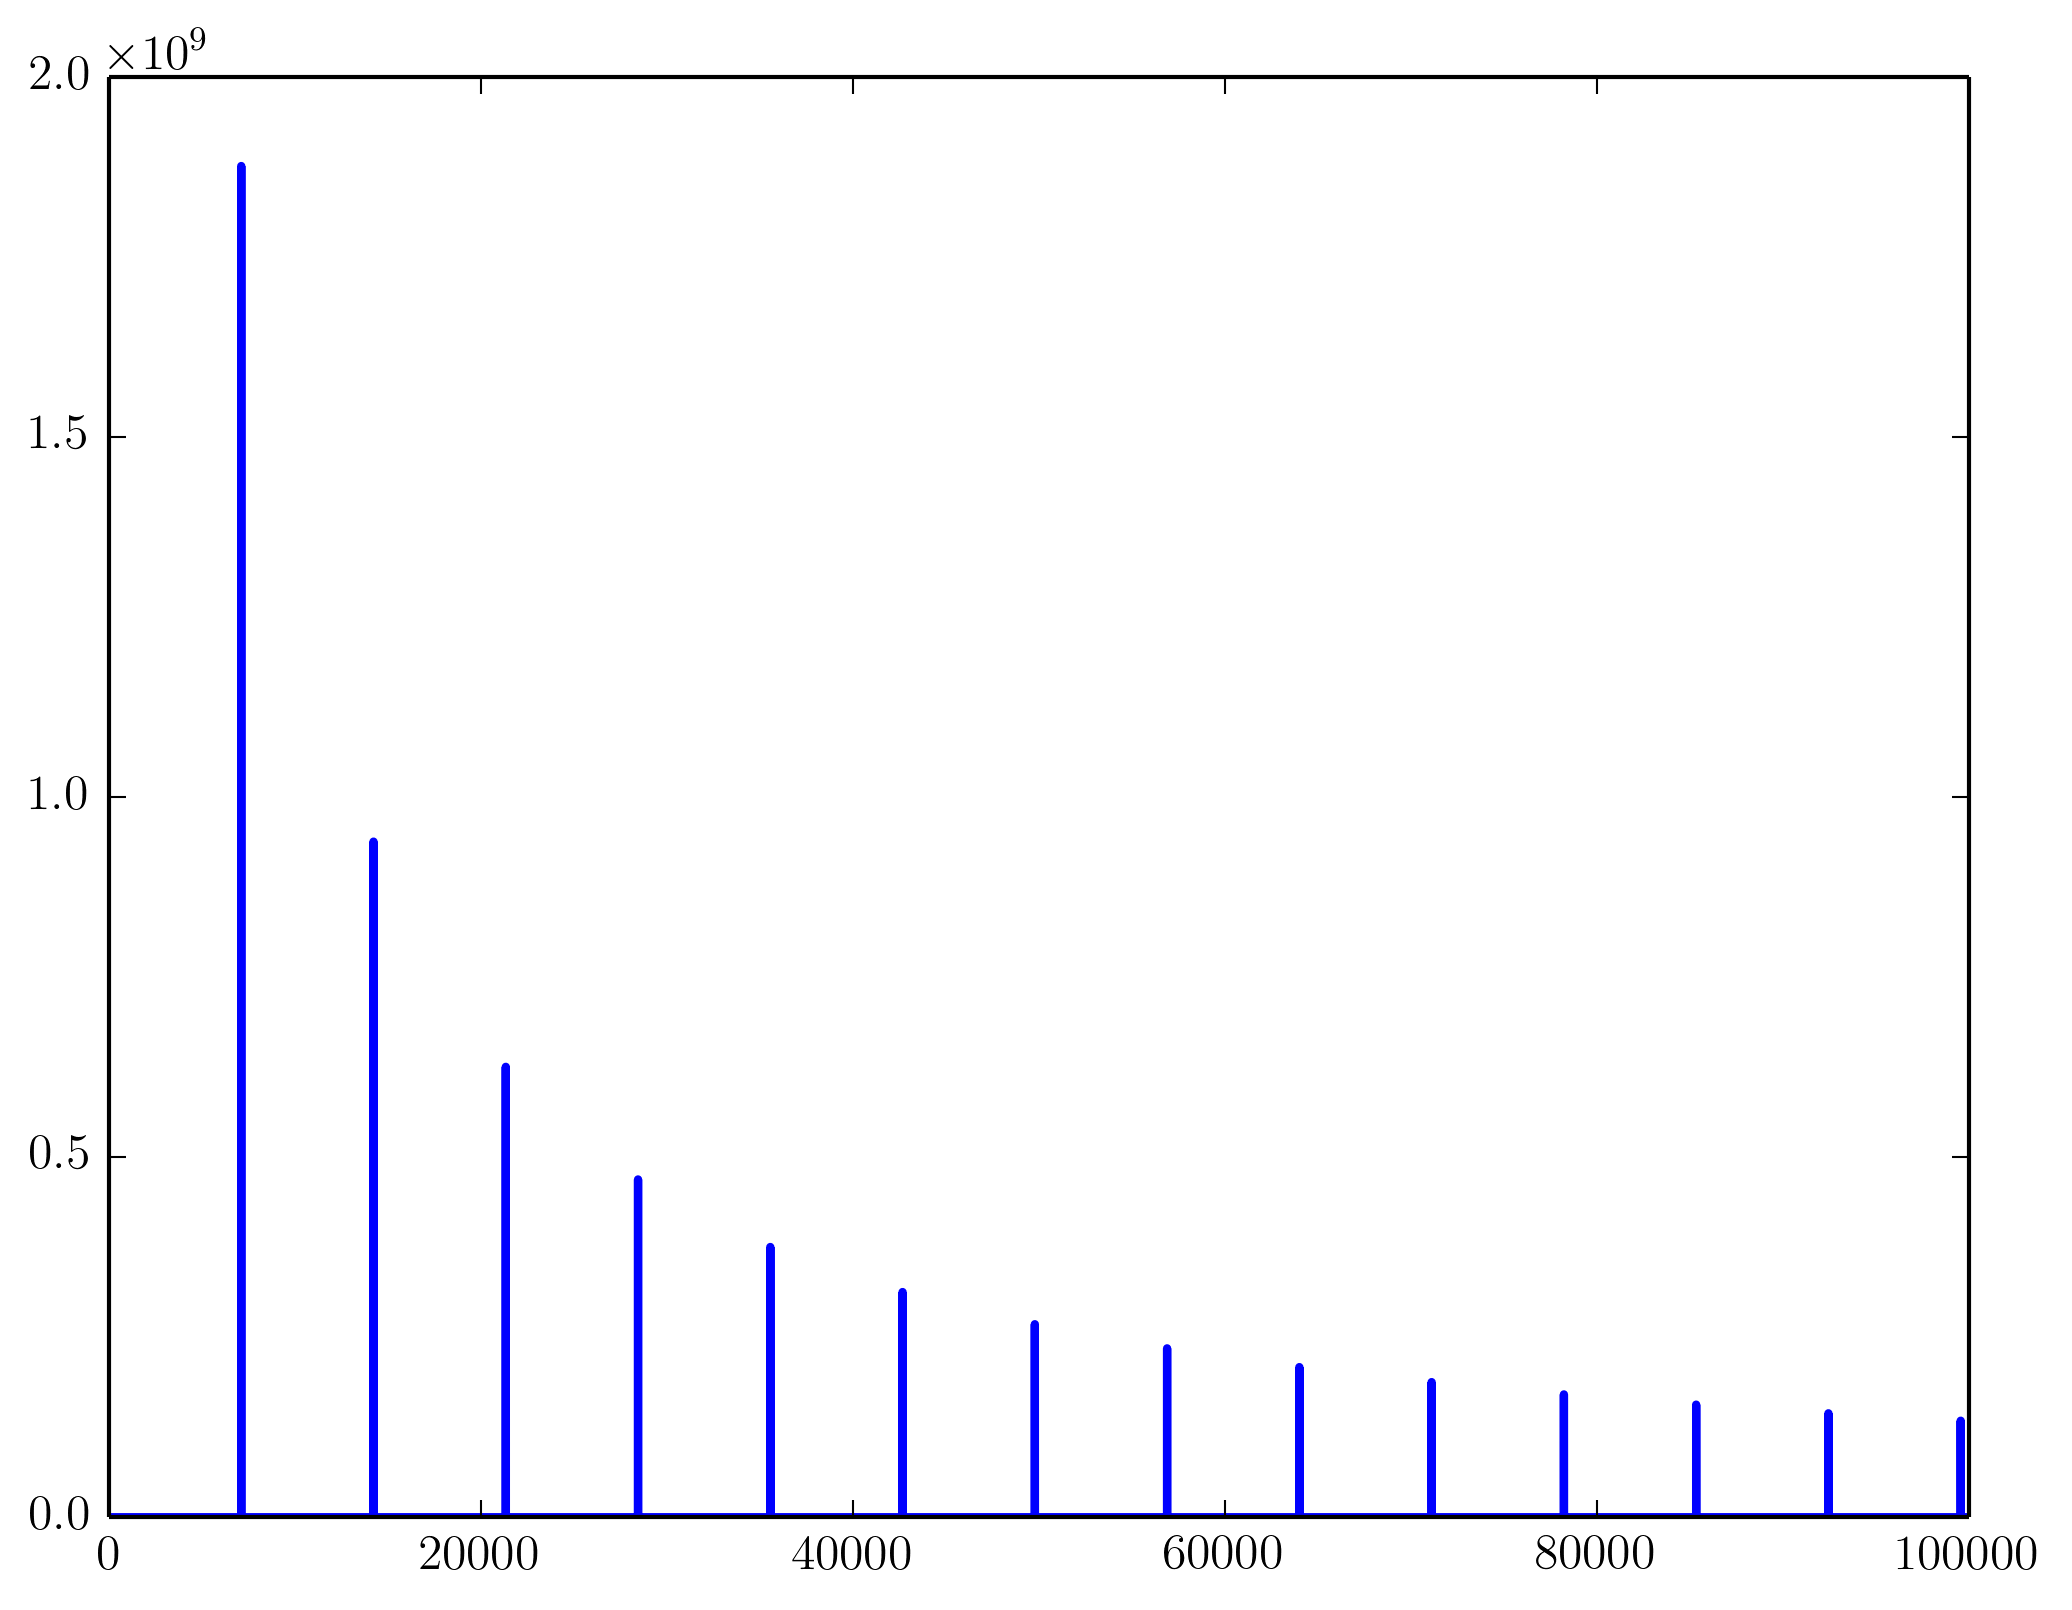
\includegraphics[width=\textwidth]{sawspec}\end{figure}

\begin{figure}[ht]\caption{Spectrum of \texttt{saw.wav} naively downsampled to 22050Hz}\label{sawspecdown}\centering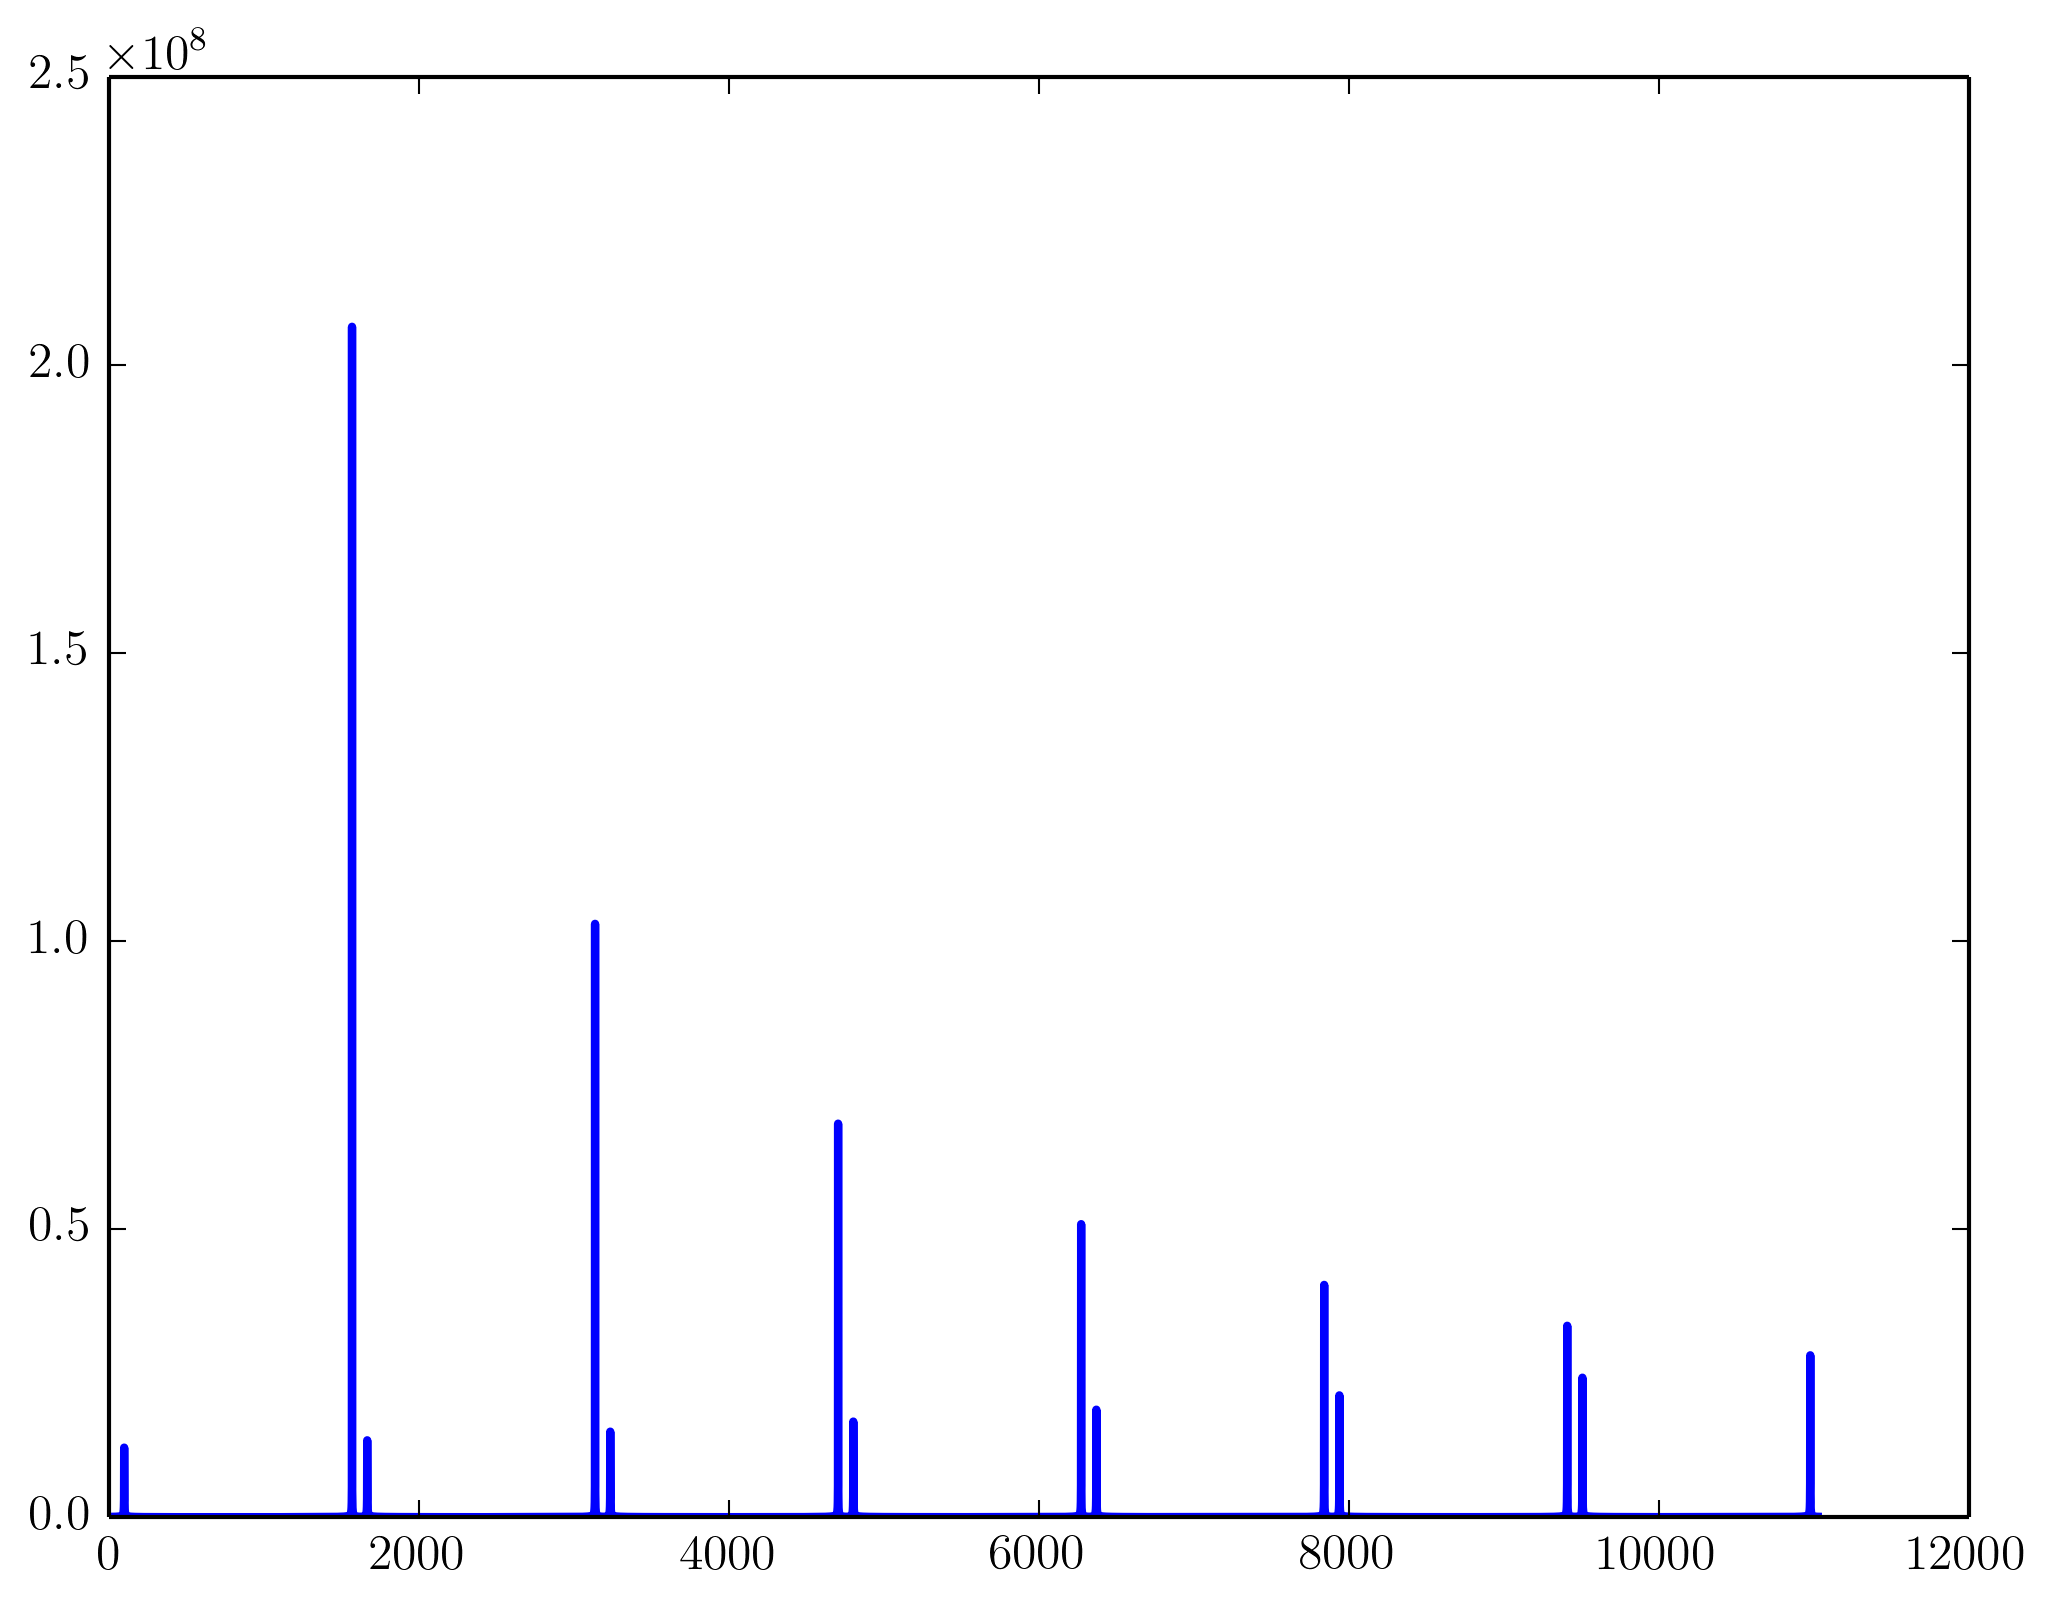
\includegraphics[width=\textwidth]{sawspecdown}\end{figure}

So, how do we downsample our signal in a way that avoids this unwanted aliasing effect? The solution is almost very simple: to start, we take the DFT of our signal, cut out the upper half of the spectrum (which can no longer be represented, after we downsample), then take the inverse DFT of the result.

Unfortunately, we're not quite done. When we say we're cutting out a set of frequencies from the spectrum, we mean we're removing those frequencies from the left half of the DFT and \emph{also} the corresponding frequencies from the right half of the DFT. So, we're actually removing a big chunk out of the \emph{middle} of the DFT and then pasting the two ends back together. We can do this as follows where in\_sig is the signal from \texttt{saw.wav}:

\begin{lstlisting}
old_rate = 44100
new_rate = 22050
in_sig = sp.float32(in_sig)
fin = fftw.fft(in_sig)
nsiz = sp.floor(in_sig.size * new_rate / old_rate)
nsizh = sp.floor(nsiz / 2)
fout = sp.zeros(nsiz)
fout = fout + 0j
fout[0:nsizh] = fin[0:nsizh]
fout[nsiz-nsizh+1:] = sp.conj(sp.flipud(fout[1:nsizh]))
out = fftw.ifft(fout)
\end{lstlisting}

There are just a couple minor problems we need to deal with before we're finished.
First, because of roundoff error, you will find that some of the entries of the \texttt{out} have (slightly) nonzero imaginary components. Therefore we should first make sure the signal is purely real,

\begin{lstlisting}
out = sp.real(out) # Take the real component of the signal
\end{lstlisting}

Second, as always, we need to rescale and cast the signal as a 16-bit integer:

\begin{lstlisting}
out = sp.int16(out/sp.absolute(out).max() * 32767)
\end{lstlisting}

\begin{figure}[ht]\caption{Spectrum of \texttt{saw.wav} correctly downsampled to 22050Hz}\label{sawspecdown2}\centering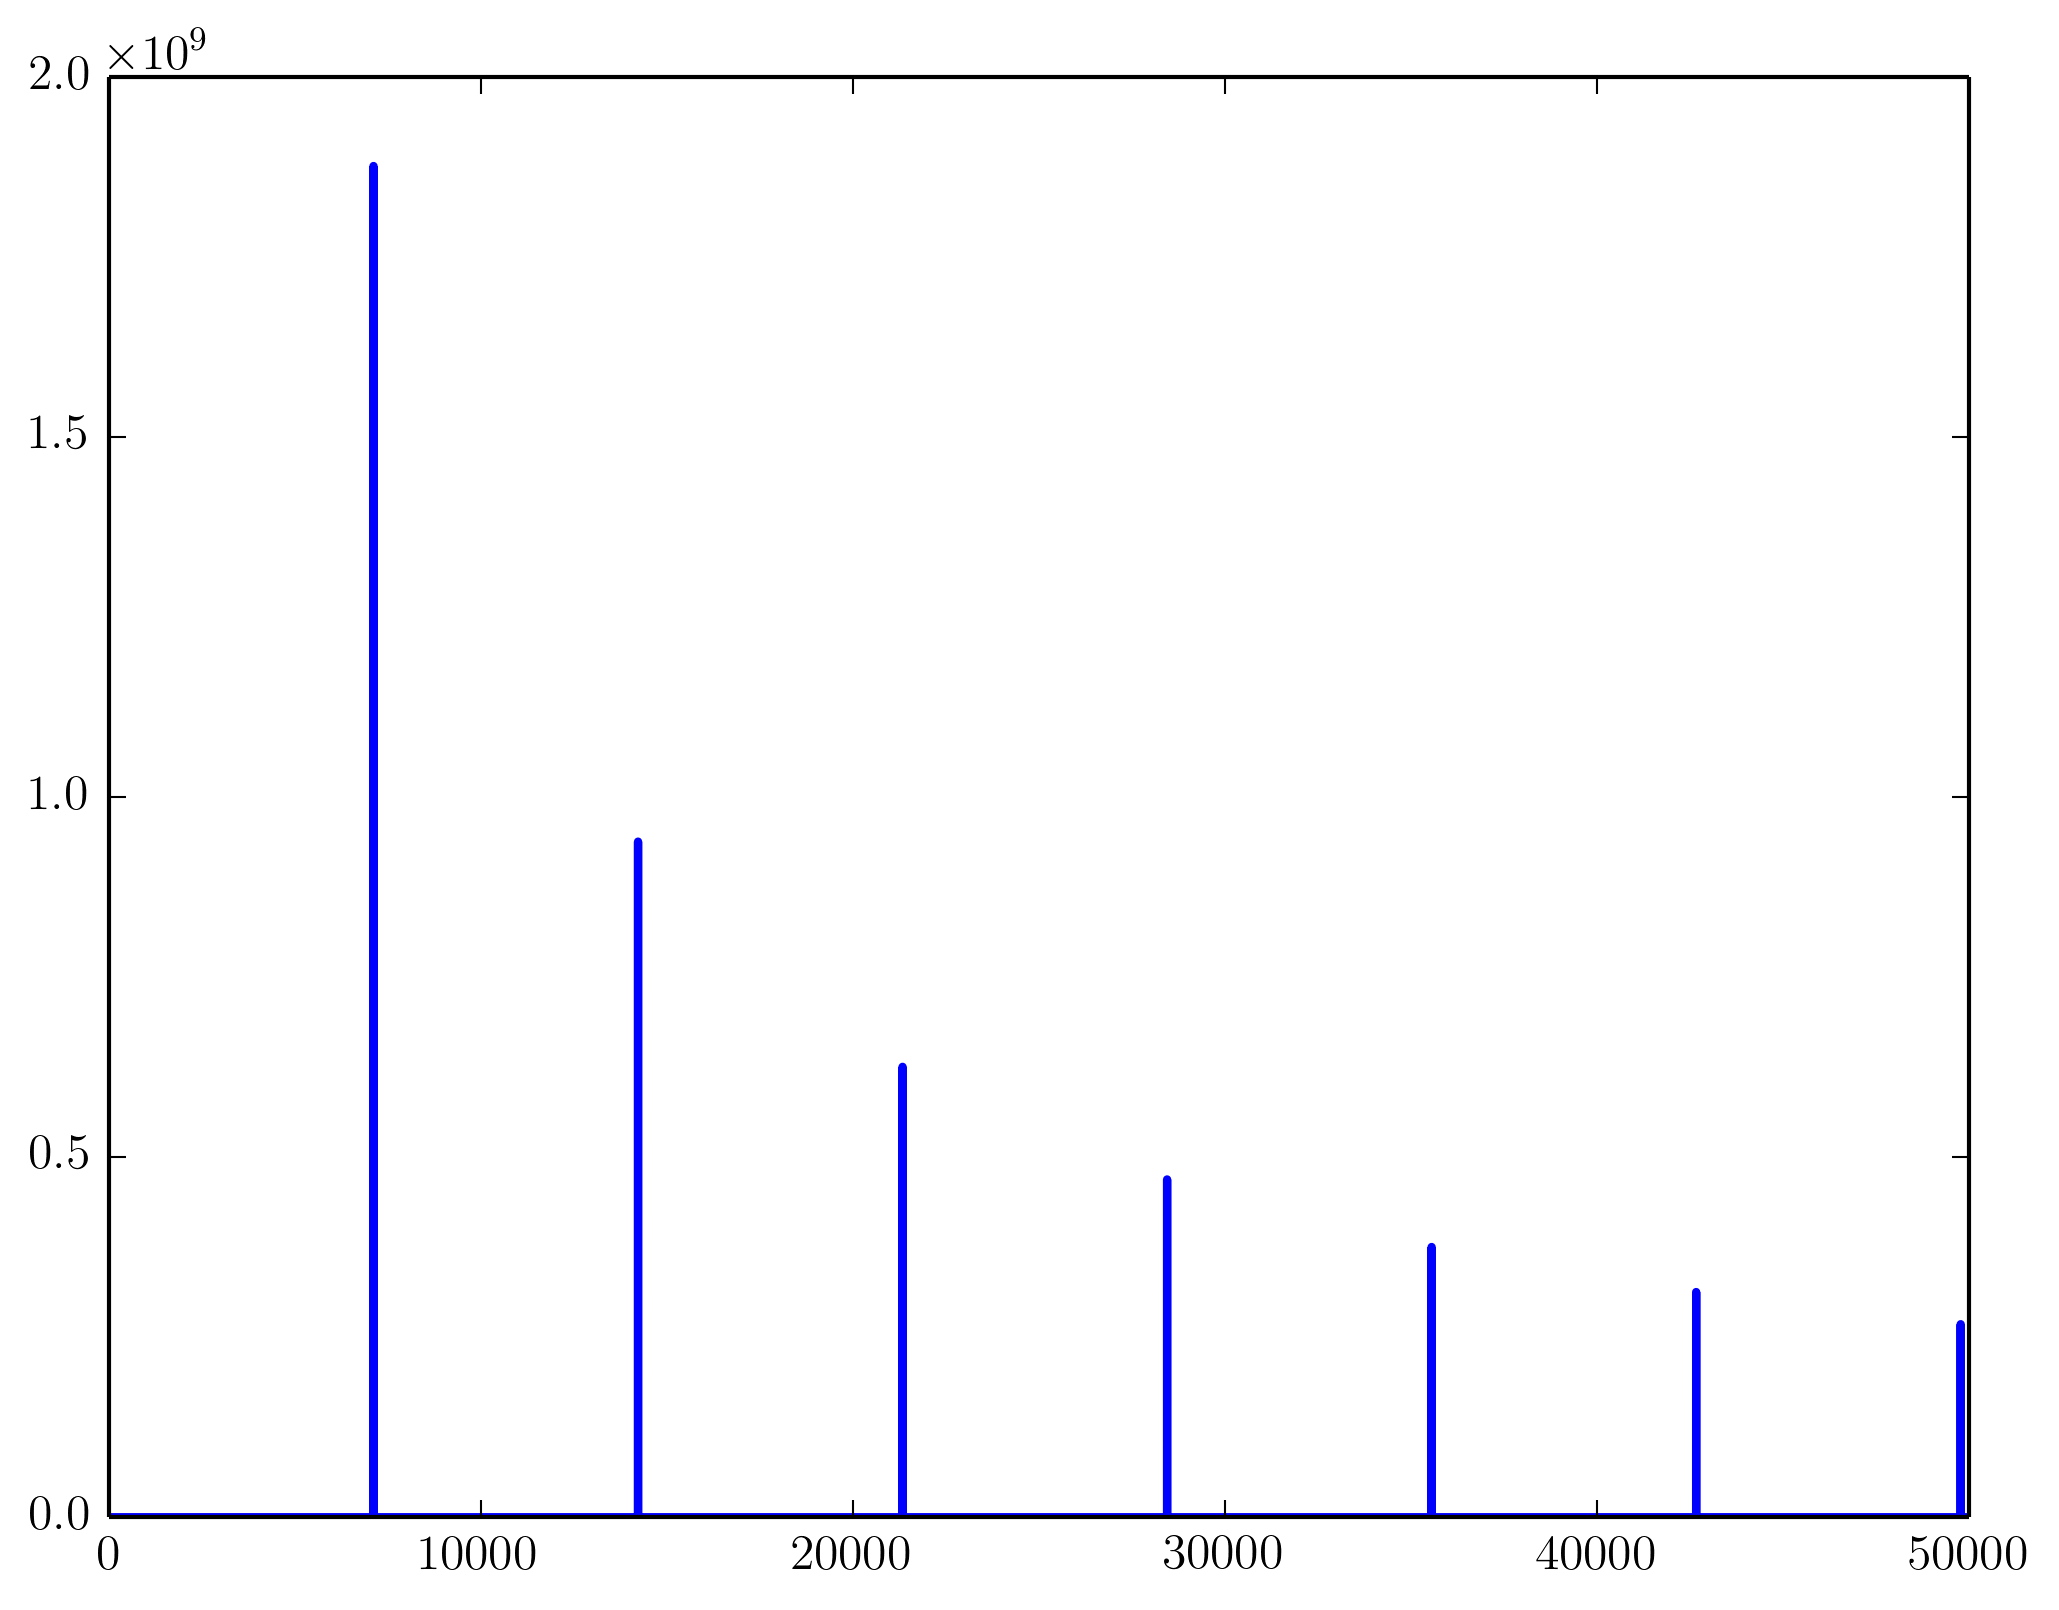
\includegraphics[width=\textwidth]{sawdownspec}\end{figure}

\begin{problem} % Problem 4
Convert \texttt{saw.wav} to a 11025Hz sampling rate. Do you notice a difference in the quality of the sound? If so, can you explain why?
\end{problem}

\begin{problem} % Problem 5
Can the technique above be used to change the sampling rate by something other than an integer factor, e.g., from 44100Hz to 36000Hz? Try it.
\end{problem}

\begin{comment}
\begin{problem}
Suppose we would like to upsample \texttt{Tada.wav} from a sampling rate of 22050Hz to 44100Hz. \begin{enumerate}
\item[(a)]
The naive way to do this would be to use linear interpolation on the original signal, i.e., the original signal would form the odd-index samples of the new signal, while the even-index samples of the new signal would be formed by taking the average of each two consecutive samples in the original signal.
Write code to carry out the upsampling in this way; plot the spectrum of the result.
What do you observe?
\item[(b)]Now write code to upsample the signal using the DFT, using a technique similar to what we did above for downsampling.
Again, plot the spectrum of the result.
Can you hear any difference between this and the result of (a)?
\end{enumerate}
\end{problem}
\end{comment}

\let\undefined\x
\let\undefined\q
\let\undefined\p
\let\undefined\v